\chapter{Implementation}
\section{Introduction}
\section{Simulation Details}
The code was written in \textit{Matlab} and is structured into multiple sections and files, to increase the modularity and readability of the code while simplifying the debugging process at the same time. The code has the following main components: 

\begin{itemize}
    \item Setup and main loop of the simulation;
    \item The drone and ARTVA classes;
    \item The trajectory replanner;
    \item The plotter (that shows graphically the simulation).
\end{itemize}

The main structure of the simulation is the following: we first perform a setup step in which we initialize the drones, the transmitting ARTVA and other useful variables and constants; then in an infinite loop we carry out all the computations that need to be performed at every time instant, such as moving the drones along their trajectories, estimating the position of the transmitting ARTVA and drawing on the screen the current state of the simulation; if some specific conditions are met we trigger the Replanner, whose job is to assign new goals to the drones; finally if we have successfully estimated the position of the transmitting ARTVA we stop the simulation. We will now discuss in more detail all the steps presented.

The simulation starts with the initialization of many variables and constants that will be useful throughout the whole experiment, such as the time step of the simulator, the kind of trajectory the drones will have to follow, the number of drones, the current time instant, whether we are in the centralized or distributed case and so on.

Then we move on to the setup step, in which we instantiate all the drones and assign them a goal as specified in the previous section about exploration strategies, then we instantiate the ARTVA by assigning it a random position inside the world region. In addition to that, we also initialize a Plotter class, whose job is to display the simulation on the screen in a separate window, but a more in-depth analysis of this component will be carried out in the following paragraph.

Finally, we move on to the main loop in which we first move the drones and then perform the estimation algorithm, directly in the main loop if we are in the centralized case or by calling the drones’ subroutine if we are in the decentralized case. In the decentralized case we also perform the Average Consensus Filter estimation as already described in a previous paragraph.\\
The next step is to check if we are satisfying the stopping criterium and in such case end the simulation: in the initialization phase we define a “threshold” value and a “control time” value so that if the estimations of the ARTVA do not move more than “threshold” meters for “control time” seconds, then we can exit the main loop and terminate. If the stopping criterium is not met, we instead need to display the next frame representing the simulation and to do so we need to pass to the Plotter class all the necessary pieces of information, such as the new positions of the drones, their updated estimations, and in the distributed case also the updated values of the ACF estimation. 

\subsection{Drone and ARTVA classes}
The simpler of the two classes is the ARTVA class, and its sole purpose is to store the position of the ARTVA itself and emit the signal received by a drone. To “emit” such a signal we use the \textit{getSignal()} function, which takes in input the position of the drone and returns a single floating-point value, that is the value of the signal perceived by the drone. To obtain such value we can use the same equation that the drones use to estimate the ARTVA, namely $y(p_k,\tau_k) = \phi^T(p_k)x(p_t)$.\\
The only difference is that in this case $x(p_t)$ is a vector of known constants that is populated as follows: 
\begin{itemize}
    \item $\bar{m}_{11} = \bar{m}_{22} = \bar{m}_{33} = 1$
    \item $\bar{m}_{12} = \bar{m}_{13} = \bar{m}_{23} = 0$
    \item $\bar{p}_t = p_t$ is now the real vector of the ARTVA position and not its estimated value
    \item $\rho = p^T_tp_t$
\end{itemize}

The drone class is instead more complex since it has to oversee both the drone’s movement and the drone’s distributed estimation tasks. Moreover, like the ARTVA class, the drone class is used to store some useful properties such as the drone’s position, state, goal and distributed estimation variables (when needed). 

Relatively to the movement task, the two most important functions are \textit{setGoal()}, that allows to specify a point in space that the drone should reach, and \textit{move()}, that allows to move the drone in small steps following either a bang-coast-bang or a bang-bang velocity profile, depending on whether the distance from the objective is big enough to allow for a coasting phase. 

Relatively to the distributed estimation task, the three most important functions are \textit{sync()}, that retrieves the information from nearby drones, \textit{estimate()}, that performs the actual distributed estimation algorithm, and \textit{ace()}, that implements the Average Consensus Filter. As a sidenote, in the estimation algorithm we used the pseudo-inverse in order to calculate $S^{-1}$.

\begin{comment}
To invert the matrix we used the pseudo-inverse, since choosing a value of $\beta = 0.999$ made the S matrix singular, and hence non-invertible.
The update of the estimation is performed by the code: \\

$\texttt{est\textunderscore X = est\textunderscore X + pinv(est\textunderscore S)*(est\textunderscore H*(est\textunderscore Y - est\textunderscore H.'*est\textunderscore X));}$\\
$\texttt{est\textunderscore S = est\textunderscore beta*est\textunderscore S + est\textunderscore H * est\textunderscore H.’;}$\\

Where:
\begin{itemize}
    \item \texttt{est\textunderscore beta} is $\beta$;
    \item \textit{pinv()} is the \textit{Matlab} function used to calculate $S^{-1}$.
\end{itemize}
\end{comment}

\subsection{Replanner}
The Replanner is a single function that manages the trajectory re-planning whenever all the drones have reached their objective. Its behavior depends on the kind of trajectory type chosen, but the main idea is to wait for all the drones to reach their first objective, which is the one that makes the drones explore the space, and then make them converge to the estimated point.\\ 
While converging to the estimated point, the space is explored further and once the drones reach their goal, a new, refined value for the estimated point is available. So once all the drones converge to their first estimated point, the Replanner sets the new, refined value as their new goal and this “looping” behavior continues until the stopping criterion of the simulation is met. 

\subsection{Plotter}
The Plotter class is the component that is responsible for the visualization of the simulation in real time: to do so, it opens a separate window at the beginning of the simulation and efficiently displays the simulation inside it. Since the draw calls of the Plotter can be the real bottleneck in the main loop of the simulation, we carefully optimized the code relative to this task so that redrawing the scene only updates the parts that changed between subsequent time-steps and everything else is kept as is.\\
It should be noted that the simulation waits a defined time-step at each loop, from which all the computational time is subtracted, so to have faster simulations. However, this does not affect the time used to comment the results or for other calculations used in the algorithm, which remains the actual time it takes the drones to converge. 

After this optimization, we managed to make the Plotter run fast enough that the simulation seems effectively in real time (since the draw calls do not run in a separate thread and therefore are blocking calls).\\
The Plotter displays:

\begin{itemize}
    \item The lines determining either the vertical lanes or the circular sectors, depending on the trajectory; 
    \item The drones, each with their own unique color to make them distinguishable;
    \item The position of the real ARTVA; 
    \item The position of the single estimation of the ARTVA, if in the centralized estimation mode; 
    \item The position of the multiple estimations of the ARTVA, each with the same color of the corresponding drone, if in the decentralized estimation mode; 
    \item The position of the multiple ACF estimations, each with the same color of the corresponding drone, if in the decentralized estimation mode. 
\end{itemize}
On a side-note, it should also be noted that the Plotter class is designed to adapt its behavior at run-time depending on the number of drones, trajectory chosen and mode of estimation.

\subsection{Stopping Criterium}
The stopping criterium was implemented right after the estimation of the ARTVA position and works in the following way: the values of those estimates are saved and used to check when the algorithm is not updating them significantly anymore. To do so, we first choose a number of time instants k representing how long the algorithm should "remain stable enough" to assess its convergence. Then we implemented a list named \textit{check} that contains k binary variables all initialized to 1: the idea is that if $check[i] = 0, \forall i \in [0,k-1]$, then in the last k time instants the estimations "did not change significantly", thus we converged to a reasonable solution and we can stop the simulation.

In the centralized case, the $check[i]$ value is set to 0 when the difference between the estimate at time \textit{i} and the estimate at time \textit{i-1} falls below a threshold decided in advance. This is the way in which we encode the fact that the current estimation "did not change significantly". If that is not the case, the variable remains 1.\\
When the \textit{check} array variable contains only 0 values, the algorithm terminates. However, an additional check is performed in this case: it is verified whether the difference between the current estimate and the estimate obtained k time instants ago falls below the threshold. This ensures that not only the estimates remained relatively stable during the control time period (i.e., subsequent changes were smaller than the threshold), but that the cumulative change was small enough to make it pointless for the algorithm to continue.

In the distributed scenario, the stopping criterium remains fundamentally unchanged. However, the chosen estimate value is based on the mean estimated by the last drone through the ACF estimation. Thanks to the high precision of the ACF performance (with differences in the order of millimeters), it is possible to select arbitrarily any drone. This selected drone then signals all others to stop the search, as the goal has been accurately estimated. We opted for the final drone rather than any other one, as in the "\textit{linear}" case the last drone covers the greatest distance, which improves its estimation performance. In the other two cases, though, the choice was irrelevant because there were no drones outperforming the others, since they all tend to travel more or less the same amount of space.
\section{Particle Swarm Optimization}
The PSO\footnote{PSO stands for Particle Swarm Optimization.} algorithm was first introduced in 1995 
\cite{PSO_original}, and it has since proven to be a powerful tool for solving various optimization problems. 
In the standard PSO algorithm, a population of particles is randomly initialized to represent potential candidate 
solutions for the optimization problem. Each particle relies on two important pieces of information: its individual 
best, referred to as \textit{pbest}, and the global best across the entire population, referred to as \textit{gbest}. 
These two values guide the search direction of all particles over the search space. The evaluation of the 
\textit{pbest} for each particle and the \textit{gbest} for the entire population is determined by the function 
that needs to be optimized.

\par In our implementation, each particle corresponds to an individual drone 
within the swarm, and the velocity and position of each drone are updated in 
accordance with the aforementioned standard PSO algorithm. Let $\mathbf{p}_i \in \mathbb{R}^2$ 
for $i = 1, 2, \dots, n$ represent the position vectors of the drones in the 2D plane, 
where $n$ is the total number of drones. The motion of each particle is governed 
by two fundamental equations: the velocity update equation (Eq.~\ref{eq:velocity}) and 
the position update equation (Eq.~\ref{eq:position}).
\begin{align}
    \mathbf{v}_{i}(t+1) &= \omega \, \mathbf{v}_{i}(t) + c_1 r_1 \left( \mathbf{pbest}_{i}(t) - \mathbf{p}_{i}(t) \right) 
    + c_2 r_2 \left( \mathbf{gbest}(t) - \mathbf{p}_{i}(t) \right) \label{eq:velocity} \\
    \mathbf{p}_{i}(t+1) &= \mathbf{p}_{i}(t) + \mathbf{v}_{i}(t+1) \label{eq:position}
\end{align}
    
where $\mathbf{p}_i$, $\mathbf{pbest}_i$, and $\mathbf{gbest}$ represent the position vector of the $i$-th particle, 
the $i$-th particle's individual best position vector, and the global best position vector, 
$\omega$ is the inertia weight, $c_1$ and $c_2$ are positive constants, and
$r_1$ and $r_2$ are random variables uniformly distributed over the interval $[0, 1]$.

\par In the standard PSO algorithm, there is only one global best particle, 
which means that only one optimal solution can be found. This limitation 
poses a challenge when dealing with our problem, where we are looking for multiple sources, 
and therefore, multiple local and global optima exist. To address this challenge, 
we employ the same strategy of a modified version of the PSO algorithm \cite{PSO_IMPORTANT}. 
In this modification, the swarm is divided into $M$ subpopulations, each tasked with exploring 
different regions of the search space. Following this idea, the \textit{gbest} is referred to as 
the best particle of each subpopulation, not as the global best particle in the whole population. 
This means that these $M$ best particles are separately able to catch different optima, at most $M$ optima.

\par The function \texttt{sort\_drones\_in\_groups} returns the number of groups and sorts the 
particles in different groups based on the following logic (see Algorithm~\ref{alg:sort_drones_in_groups}):
\begin{algorithm}[H]
    \caption{\texttt{sort\_drones\_in\_groups} (MATLAB function)}\label{alg:sort_drones_in_groups}
    \begin{algorithmic}[1]
    \State \textbf{Inputs:}
    \State $n\_drones$: Number of drones available for assignment
    \State $n\_sources$: Number of sources to which drones need to be assigned
    \State \textbf{Outputs:}
    \State $group\_indices$: A vector of size $n\_drones$ indicating the assigned group
    \State $n\_groups$: The obtained number of groups
    \If{$n\_particles > n\_sources$}
        \State Assign at least one particle to each group, following mathematical order
        \State Randomly assign remaining particles to existing groups
    \ElsIf{$n\_particles = n\_sources$}
        \State Assign each particle to a unique group
    \Else
        \State Orderly assign particles up to $n\_drones$
    \EndIf
    \State Set the number of groups: $n\_groups = max(group\_indices)$
    \end{algorithmic}
\end{algorithm}

\par Note that the function \texttt{sort\_drones\_in\_groups} ensures the creation of sufficient groups 
for the localization of multiple sources only when the number of drones is equal to or greater than 
the number of sources.

\section{Exploration phase}
\par Unlike the modified PSO algorithm, in our implementation, the drones are not randomly initialized. 
At the start of the simulation, all drones are located at the origin of the search space. 
An Exploration Phase begins where the PSO algorithm is not yet employed. 
During this phase, the drones move according to predefined trajectories at maximum speed $v_{\text{max}}$. 
The trajectories are determined based on the number of drones and follow a radial pattern, as shown in Figure \ref{fig:exploration_pattern}. 
The drones follow these trajectories until they have covered a distance $travel\_distance$ equivalent to half the boundary of the search space.
The goal each drone needs to reach is computed using the following Algorithm~\ref{alg:exploration_goals}:

\begin{algorithm}[H]
    \caption{\texttt{exploration\_goals} (MATLAB function)} \label{alg:exploration_goals}
    \begin{algorithmic}[1]
        \State \textbf{Input:} $n\_{drones}$, $x\_{max}$
        \State \textbf{Output:} $goals$ 
        \State Initialize an empty array $goals$
        \State Set $angle\_step = 360 / n\_{drones}$
        \State Set $travel\_distance = x\_{max} / 2$ 
        \For{each drone $i = 1, 2, \dots, n\_{drones}$}
            \State Get angle for the current drone: $drone\_angle = i \cdot angle\_step$
            \State Calculate slope: $m = \tan(\texttt{deg2rad}(drone\_angle))$
            \If{$drone\_angle > 315$ \textbf{or} $drone\_angle \leq 45$} 
                \State $goal = [travel\_distance, m \cdot travel\_distance]$ \Comment{1st quadrants}
            \ElsIf{$drone\_angle > 45$ \textbf{and} $drone\_angle \leq 135$}
                \State $goal = [travel\_distance / m, travel\_distance]$ \Comment{2nd quadrant}
            \ElsIf{$drone\_angle > 135$ \textbf{and} $drone\_angle \leq 225$}
                \State $goal = [-travel\_distance, m \cdot -travel\_distance]$ \Comment{3rd quadrant}
            \ElsIf{$drone\_angle > 225$ \textbf{and} $drone\_angle \leq 315$}
                \State $goal = [-travel\_distance / m, -travel\_distance]$ \Comment{4th quadrant}
            \EndIf
            \State Store the goal for drone $i$ in $goals[i]$
        \EndFor
        \State Return $goals$
    \end{algorithmic}
\end{algorithm}

where $angle\_step$ is the angular increment to uniformly divide the space, $drone\_angle$ represents the angle assigned to each drone, determining its trajectory, 
while $m$ is the slope of the trajectory calculated from the drone's angle. 

\begin{figure}
    \centering
    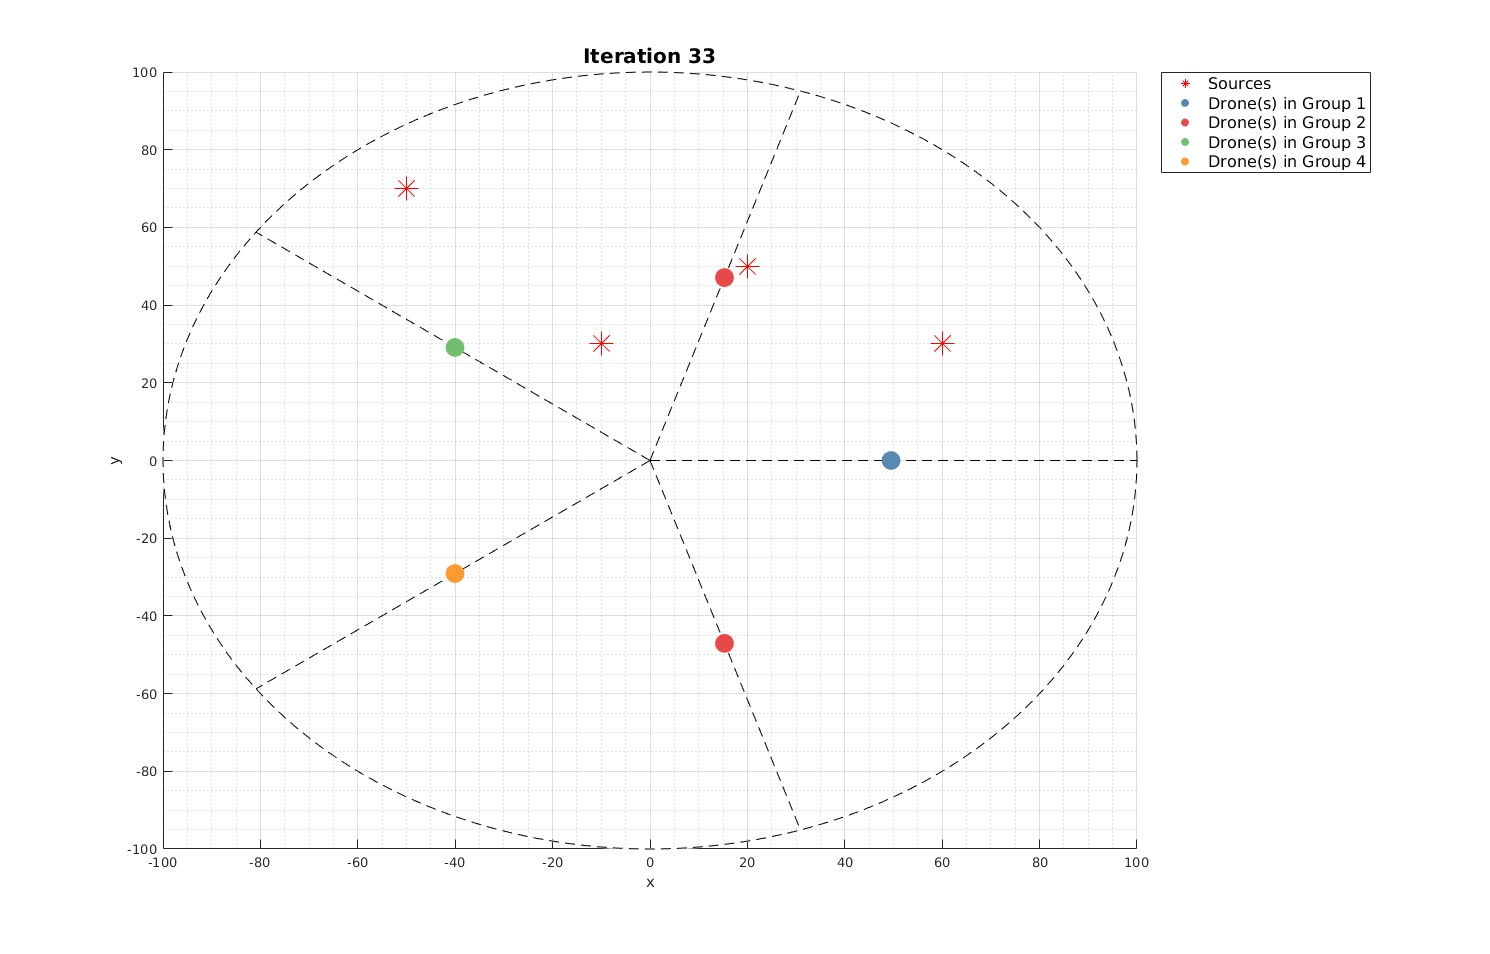
\includegraphics[width=\textwidth]{images/exploration_pattern.jpg} 
    \caption{Radial exploration pattern for 5 drones at the end of the Exploration Phase.}
    \label{fig:exploration_pattern}
\end{figure}

\section{Exploitation Phase}
\subsection{Velocity Update}
At each time step, the velocity update of the standard PSO algorithm is modified in order to favor the complete 
exploration of the search space and to avoid premature convergence to local maxima, where a source is not present. 
A uniform random noise is added to the velocity of each particle to achieve a \textit{persistence of excitation},
allowing every drone to explore new and different directions, 
as described in the following formula:
\[
\mathbf{v}_i = \mathbf{v}_i + \beta \cdot \mathbf{r} \cdot ||\mathbf{v}_i||
\] \label{eq:persistence_of_excitation}
where:
\begin{itemize}
    \item \(\beta\) is an hyperparameter chosen in the [0,1] range.
    \item \(\mathbf{r} \sim \mathcal{U}(-1, 1)\) represents a random vector where each component is uniformly distributed between \(-1\) and \(1\).
    \item \(||\mathbf{v}_i||\) is the magnitude of the velocity vector of particle \(i\).
\end{itemize}
Furthermore, not only because of the physical velocity limitations of the drones, but also to ensure smoother updates 
and prevent instability due to excessive velocity, we clamp the velocity of each drone 
to a maximum value \(v_{\text{max}}\):
\[
\mathbf{v}_i = 
\begin{cases} 
v_{\text{max}} \cdot \frac{\mathbf{v}_i}{\|\mathbf{v}_i\|}, & \text{if } \|\mathbf{v}_i\| \geq v_{\text{max}} \\
\mathbf{v}_i, & \text{otherwise}
\end{cases}
\] \label{eq:velocity_clamping}


\subsection{Exclusion Zone Mechanism}
An additional modification to the standard PSO algorithm 
is the introduction of an exclusion zone mechanism.
This mechanism prevents multiple drones from focusing 
on the same source. It involves defining regions that 
other particles should avoid, promoting better exploration 
and reducing redundancy in source detection. The exclusion 
zone mechanism involves several key parts:
\begin{itemize}
    \item \textbf{Detection}: A drone sets its exclusion zone 
    when it identifies a source with a signal strength (NSS) 
    exceeding a predefined threshold.
    \item \textbf{Sharing}: The drone shares the position of 
    its exclusion zone with neighboring drones.
    \item \textbf{Checking}: Each drone continuously checks 
    its position against all shared exclusion zones.
    \item \textbf{Avoidance}: If a drone finds itself within 
    a shared exclusion zone, it moves away from the zone 
    following a calculated escape vector.
\end{itemize}

\subsubsection{Detection}
Each drone establishes an exclusion zone when it detects a 
source, meaning it has computed an NSS higher than a certain 
threshold. The exclusion zone is defined as a circular area 
centered around the position of the drone where the source 
was detected. The radius of this zone is a fixed parameter, 
chosen experimentally, which determines the \textit{resolution} 
of the algorithm.

\subsubsection{Sharing}
Our algorithm favors a decentralized approach, which is useful 
in scenarios where communication between drones is not always 
possible or easy. A drone can communicate with another when 
they are less than 5 meters apart (\(r_{\text{comm}}\)).
When a drone identifies a source 
and sets its exclusion zone, it shares the estimated position 
of the source with the drones within the communication range. 
Each drone maintains a list of exclusion zones that it has 
received from others. This sharing process helps the swarm 
avoid redundant exploration around already identified sources.

\subsubsection{Avoidance}
When a drone detects that it is within the radius of a shared 
exclusion zone, it is programmed to move away from it. 
The drone computes a new goal position where it needs to go, far from the 
exclusion zone . After it reaches the goal, 
the PSO algorithm resumes, searching for a new source 
in a different area of the space.

The goal position is calculated using the vector joining 
the exclusion zone center \(\mathbf{c}\) and the current 
position of the drone \(\mathbf{p}_{\text{in\_zone}}\), when the drone finds itself 
in an exclusion zone. The formula is given by:

\[
\mathbf{d} = \mathbf{c} - \mathbf{p}_{\text{in\_zone}}
\]
\[
\mathbf{p}_{\text{goal}} = \mathbf{p}_{\text{in\_zone}} + \alpha \frac{\mathbf{d}}{\|\mathbf{d}\|}
\] \label{eq:move_away}

where:
\begin{itemize}
    \item \(\mathbf{d}\): Direction vector from the exclusion 
    zone center to the drone's position.
    \item \(\alpha\): Step size parameter, determining the 
    distance the drone should travel away from the exclusion zone.
    \item \(\mathbf{p}_{\text{goal}}\): Updated goal position of the drone.
    \item \(\|\mathbf{d}\|\): Norm (magnitude) of the direction 
    vector \(\mathbf{d}\), used to normalize the direction.
\end{itemize}
This calculation ensures that the drone moves directly away 
from the exclusion zone and covers a distance proportional 
to \(\alpha\). 
\\

The exclusion zone mechanism allows the swarm 
to adaptively adjust its search strategy based on the locations 
of previously detected sources, leading to faster convergence 
and improved accuracy in multi-source localization.
Finally, we can present the complete modified PSO algorithm in 
Algorithm \ref{alg:PSO}: 
\begin{algorithm}
    \caption{Particle Swarm Optimization for Multi-Source Localization}\label{alg:PSO}
    \begin{algorithmic}[1]
        \State \textbf{Initialize} drones' positions to the center of the search space.
        \State \textbf{Initialize} group best positions \( G_{\text{best}} \) and values \(\textit{NSS}_{\text{best}}\).
        \State \textbf{Assign} each drone to a group using function \ref{alg:sort_drones_in_groups}.
        
        \State \textbf{Exploration Phase}:
        \State \textbf{Compute} exploration goals using function \ref{alg:exploration_goals}.
        \For{each drone \( i \)}
            \State \textbf{Do}: reach goal.
        \EndFor

        \State \textbf{Exploitation Phase}:
        \For{each iteration \( t = 1 \) to \( n_{iters} \)}
            \For{each drone \( i \)}
                \State \textbf{Update} velocity using standard PSO formula as in Eq.\eqref{eq:velocity}.
                \State \textbf{Apply} persistence of excitation as in Eq. \eqref{eq:persistence_of_excitation}.
                \State \textbf{Limit} velocity to \( v_{\text{max}} \) as in Eq. \eqref{eq:velocity_clamping}.
                \State \textbf{Update} position as in Eq. \eqref{eq:position}.
                \State \textbf{Apply} boundary conditions to keep \(\mathbf{p}_i(t+1)\) within search bounds.
                
                \For{each other drone \( j \neq i \)}
                    \If{\(\|\mathbf{p}_i(t+1) - \mathbf{p}_j(t+1)\| \leq r_{\text{comm}}\)}
                        \If{\(\text{NSS}_{i}\) or \(\text{NSS}_{j} > \text{threshold}\)}
                            \State \textbf{Share} exclusion zones between drones \( i \) and \( j \).
                        \EndIf
                    \EndIf
                \EndFor
                
                \State \textbf{Check} if drone \( i \) is within an exclusion zone.
                \If{drone \( i \) is in an exclusion zone}
                    \If{drone \( i \) is not alone in its group}
                        \State \textbf{Reassign} drone \( i \) to a new group.
                        \State \textbf{Initialize} \( G_{\text{best}} \) and \(\textit{NSS}_{\text{best}}\) of the new group.
                    \EndIf
                    \State \textbf{Move} away from exclusion zone as in Eq. \eqref{eq:move_away}.
                    \State \textbf{Reset} personal best \(\mathbf{p}_{\text{best}, i}\).
                    \State \textbf{Set} drone \( i \) inertia \(\omega = 0\).
                \Else
                    \State \textbf{Evaluate} NSS at \(\mathbf{p}_i(t+1)\).
                    \If{current NSS \( > \) personal best NSS}
                        \State \textbf{Update} personal best \(\mathbf{p}_{\text{best}, i}\).
                    \EndIf
                    \If{current NSS \( > \) group best NSS}
                        \State \textbf{Update} group best \( G_{\text{best}} \).
                    \EndIf
                \EndIf
            \EndFor
        \EndFor
        
        \State \textbf{Return} \( G_{\text{best}} \).
    \end{algorithmic}
\end{algorithm}
Note that the inertia of a drone that has found a source is set to zero (\(\omega = 0\)), increasing
convergence speed.
Throughout the process, each drone updates its personal 
and group best positions based on newly evaluated NSS 
values, like in the standard PSO algorithm. The final output is the set of best estimates 
\( G_{\text{best}} \), composed of the best estimated position of a source by each group.